\chapter{System Evaluation}
This chapter evaluates the TrafficVision project against the objectives set out in the introduction. Here presenting the results obtained from the system's operation and discuss its strengths and weaknesses. This evaluation serves as a platform to demonstrate critical thinking in relation to the project and its outcomes.

\section{Objective Alignment}
The primary objectives of TrafficVision were to provide real-time traffic monitoring, enhance public transportation system reliability and improve user engagement through interactive features. The following sections detail how the system has met these objectives and highlight areas for further development.

\section{Real-Time Traffic Monitoring}
One of TrafficVision's core objectives was to implement real-time traffic monitoring. The system's ability to process and display live traffic conditions is illustrated in Figure \ref{fig:videoProcessing}.

\begin{figure}[H]
    \centering
    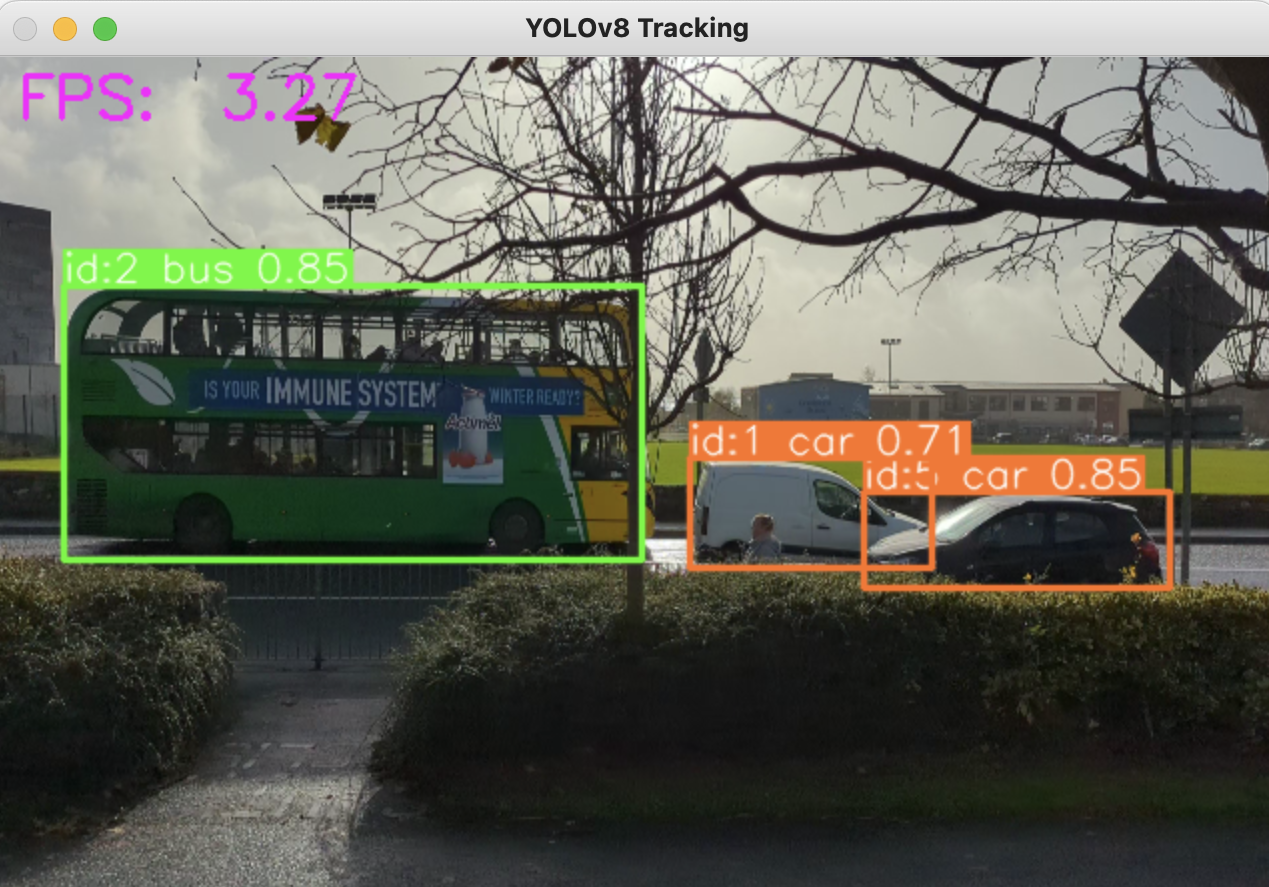
\includegraphics[width=1\linewidth]{images/videoProcessing.png}
    \caption{TrafficVision's real-time traffic monitoring interface demonstrating vehicle detection and tracking.}
    \label{fig:videoProcessing}
\end{figure}

The system successfully identifies and tracks vehicles with high accuracy and low latency, as shown in the terminal outputs in Figure \ref{fig:pythonTerminal}. However, one weakness observed is the dependency on good lighting conditions for optimal performance, which could be addressed with enhanced image preprocessing techniques or the integration of infrared camera feeds for night-time monitoring.  Future enhancements for the TrafficVision real-time monitoring system may include the integration of additional data sources such as traffic cameras across different locations, which would provide a more comprehensive traffic analysis. Additionally, machine learning techniques could be employed to predict traffic conditions based on historical data, providing users with not only the current state of traffic but also an intelligent forecast of short-term changes.

\begin{figure}[H]
    \centering
    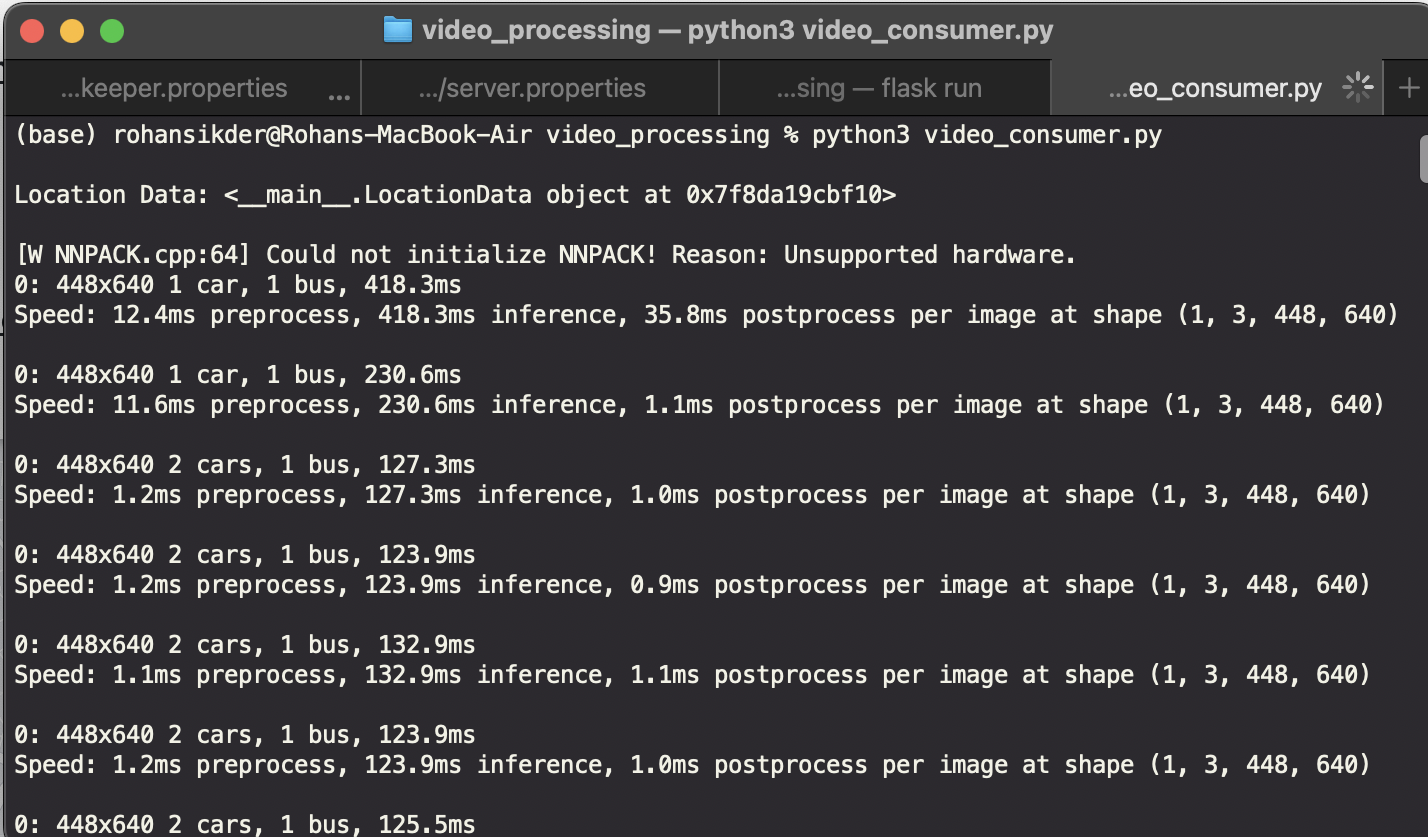
\includegraphics[width=1\linewidth]{images/pythonTerminal.png}
    \caption{Performance metrics of the TrafficVision system captured from the terminal output.}
    \label{fig:pythonTerminal}
\end{figure}

\section{Public Transportation System Reliability}

Enhancing the reliability of public transportation was another key objective. TrafficVision contributes to this by analyzing bus punctuality, as depicted in Figure \ref{fig:busUI}. The graph shows the frequency of bus appearances and can be used to assess punctuality against the schedule.

\begin{figure}[H]
    \centering
    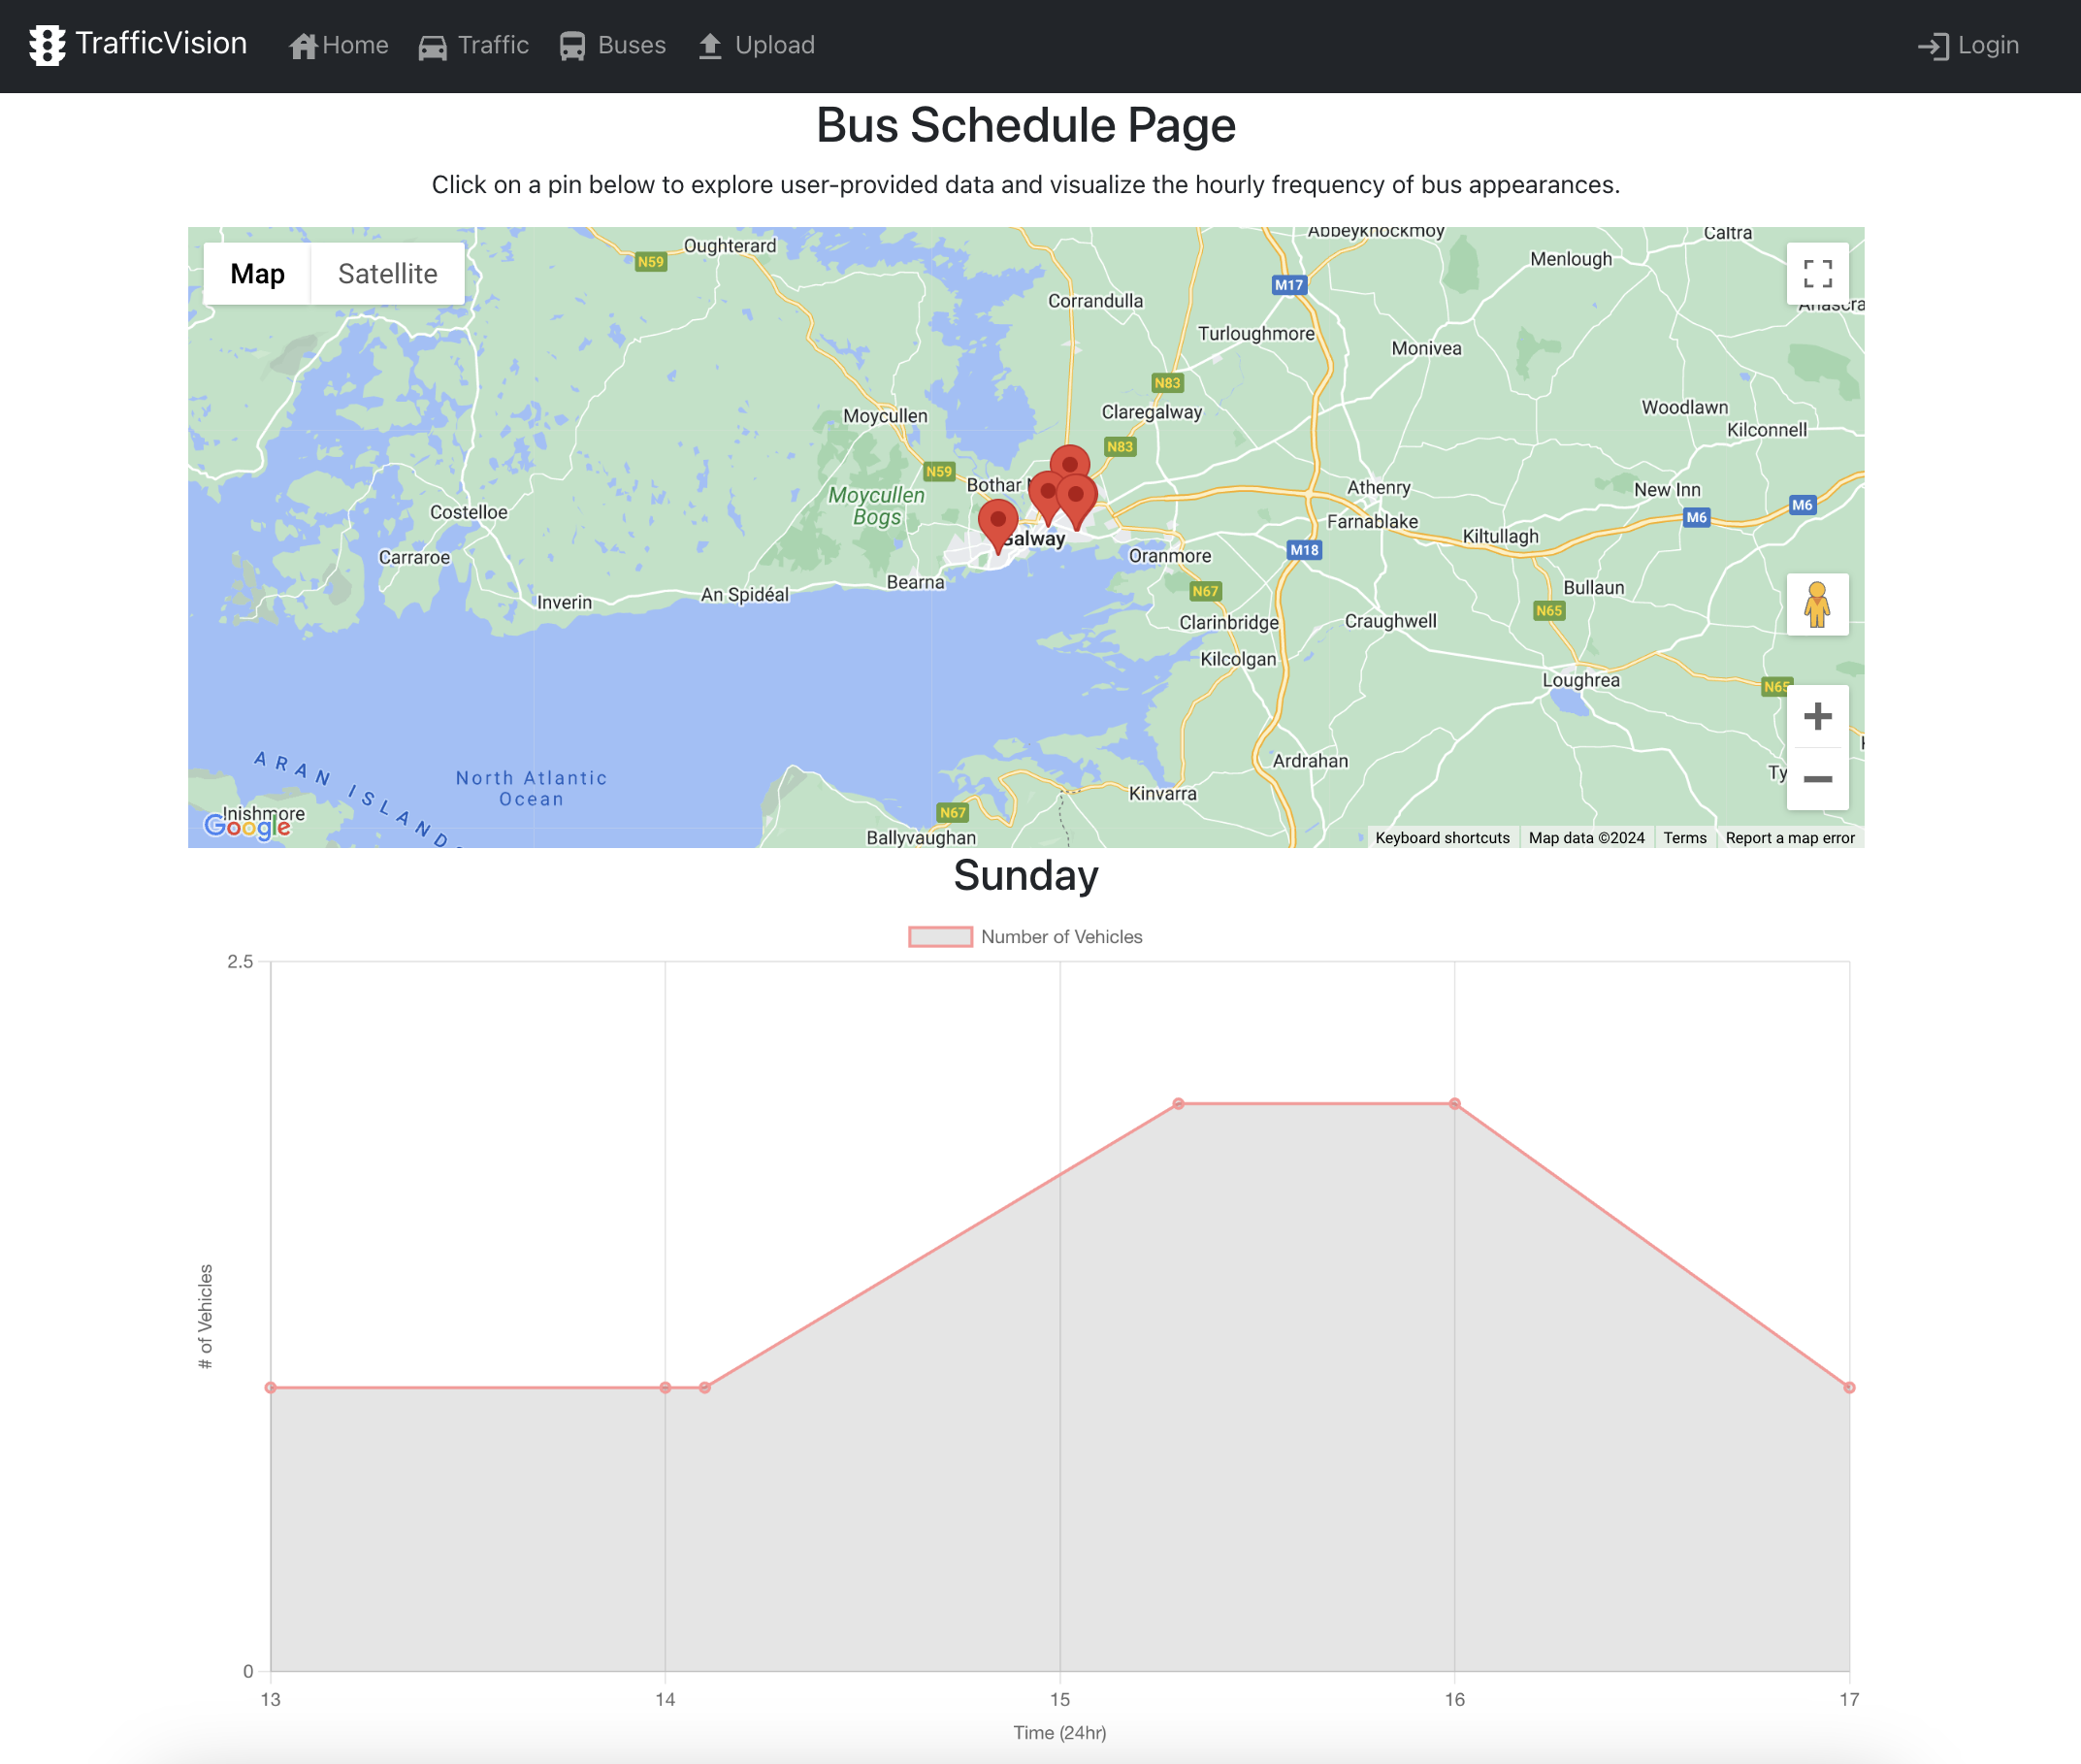
\includegraphics[width=\linewidth]{images/busUI.png}
    \caption{Visualization of bus schedule adherence using TrafficVision's data analytics.}
    \label{fig:busUI}
\end{figure}

While the system effectively records bus frequencies, the strength of the data is dependent on the quantity and quality of user submissions. This represents a limitation in data collection that could potentially be overcome with more widespread user participation or the incorporation of official transit data feeds.

\section{Integration Challenges with Transport for Ireland API}
The implementation of the Transport for Ireland API into the TrafficVision system was not a option due to the lack of documentation and complexity of the API. The API, which provides real-time bus schedules with arrival and departure times, was critical to compare how late buses were.

After research on attempts to integrate this API due to the significant challenges faced, including the API being oriented towards internal use by Transport for Ireland. Restricted accessibility making it not suitable for the TrafficVision project.

Alternative data sources were looked at that could provide accurate real time bus schedules along with departure and arrival times. However, no suitable alternatives were identified that satisfied the project's specific accessibility, reliability and integration needs.

\section{User Engagement and Interaction}

User engagement is critical for crowd-sourced platforms like TrafficVision. The UI and UX are designed to be intuitive and engaging, as evident in the system's login page (Figure \ref{fig:loginUI}) and the traffic upload feature (Figure \ref{fig:uploadUI}).

\begin{figure}[H]
    \centering
    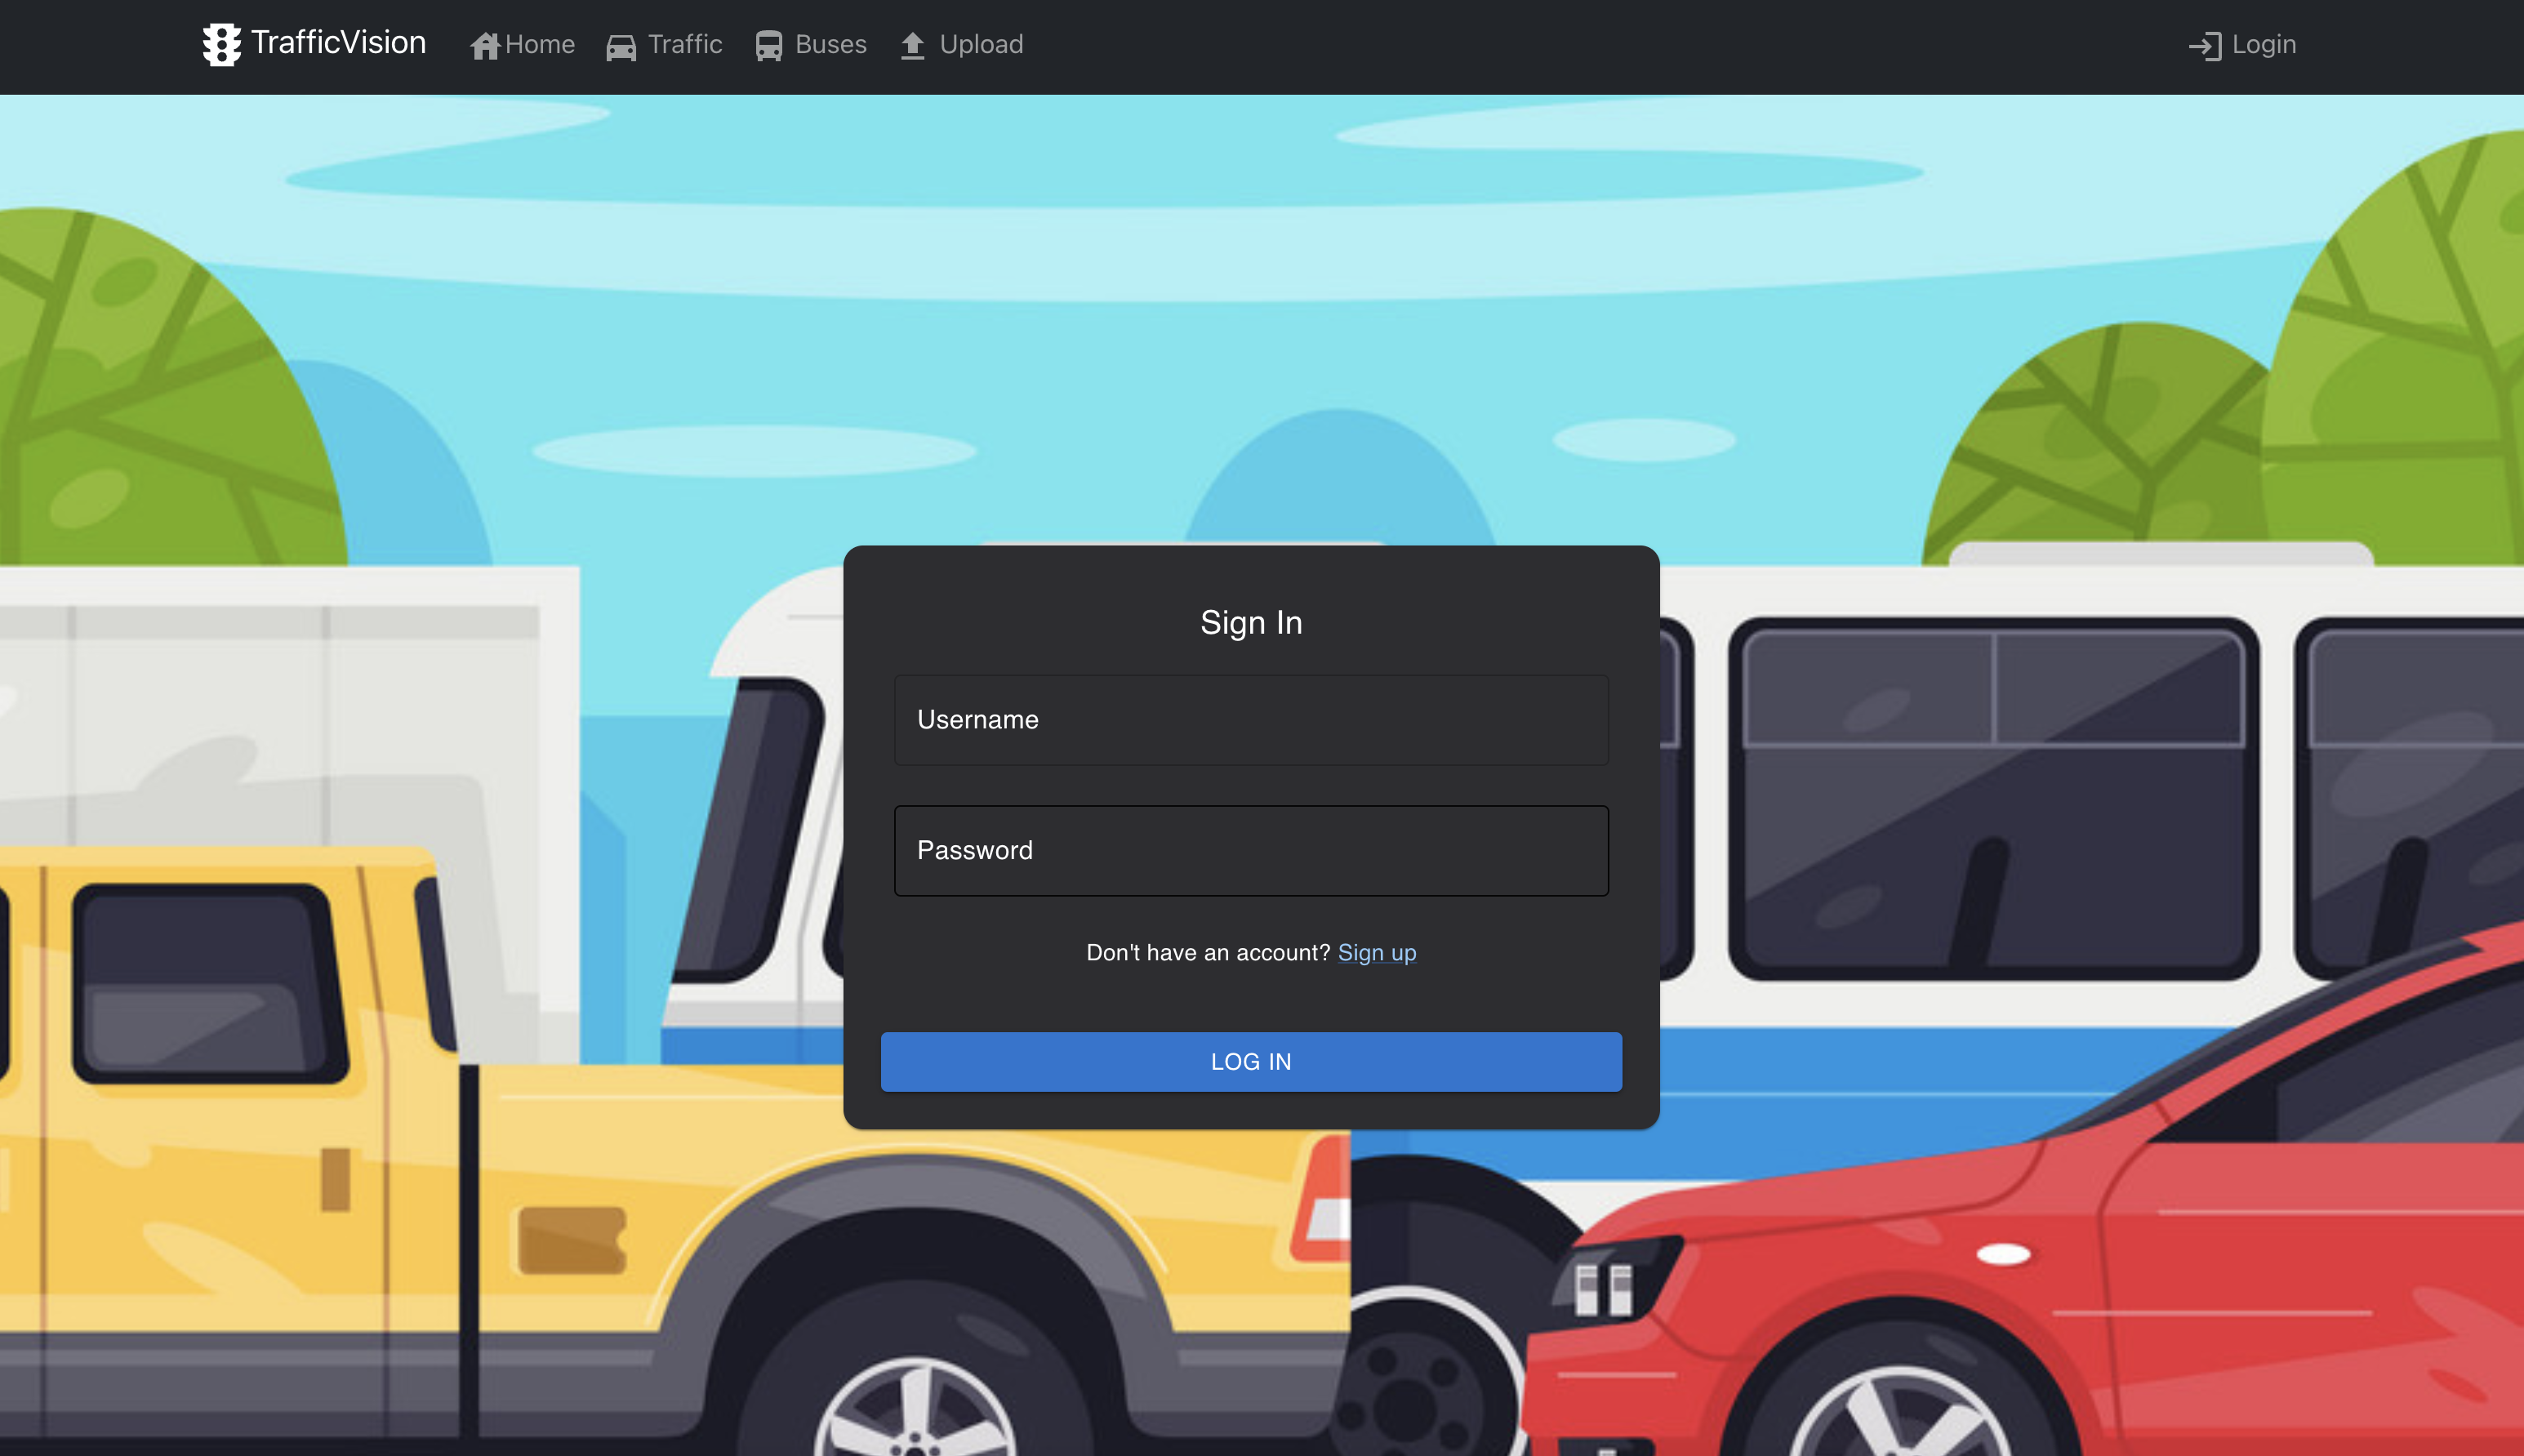
\includegraphics[width=\linewidth]{images/loginUI.png}
    \caption{The login page of TrafficVision, showcasing the system's user-friendly interface.}
    \label{fig:loginUI}
\end{figure}

\begin{figure}[H]
    \centering
    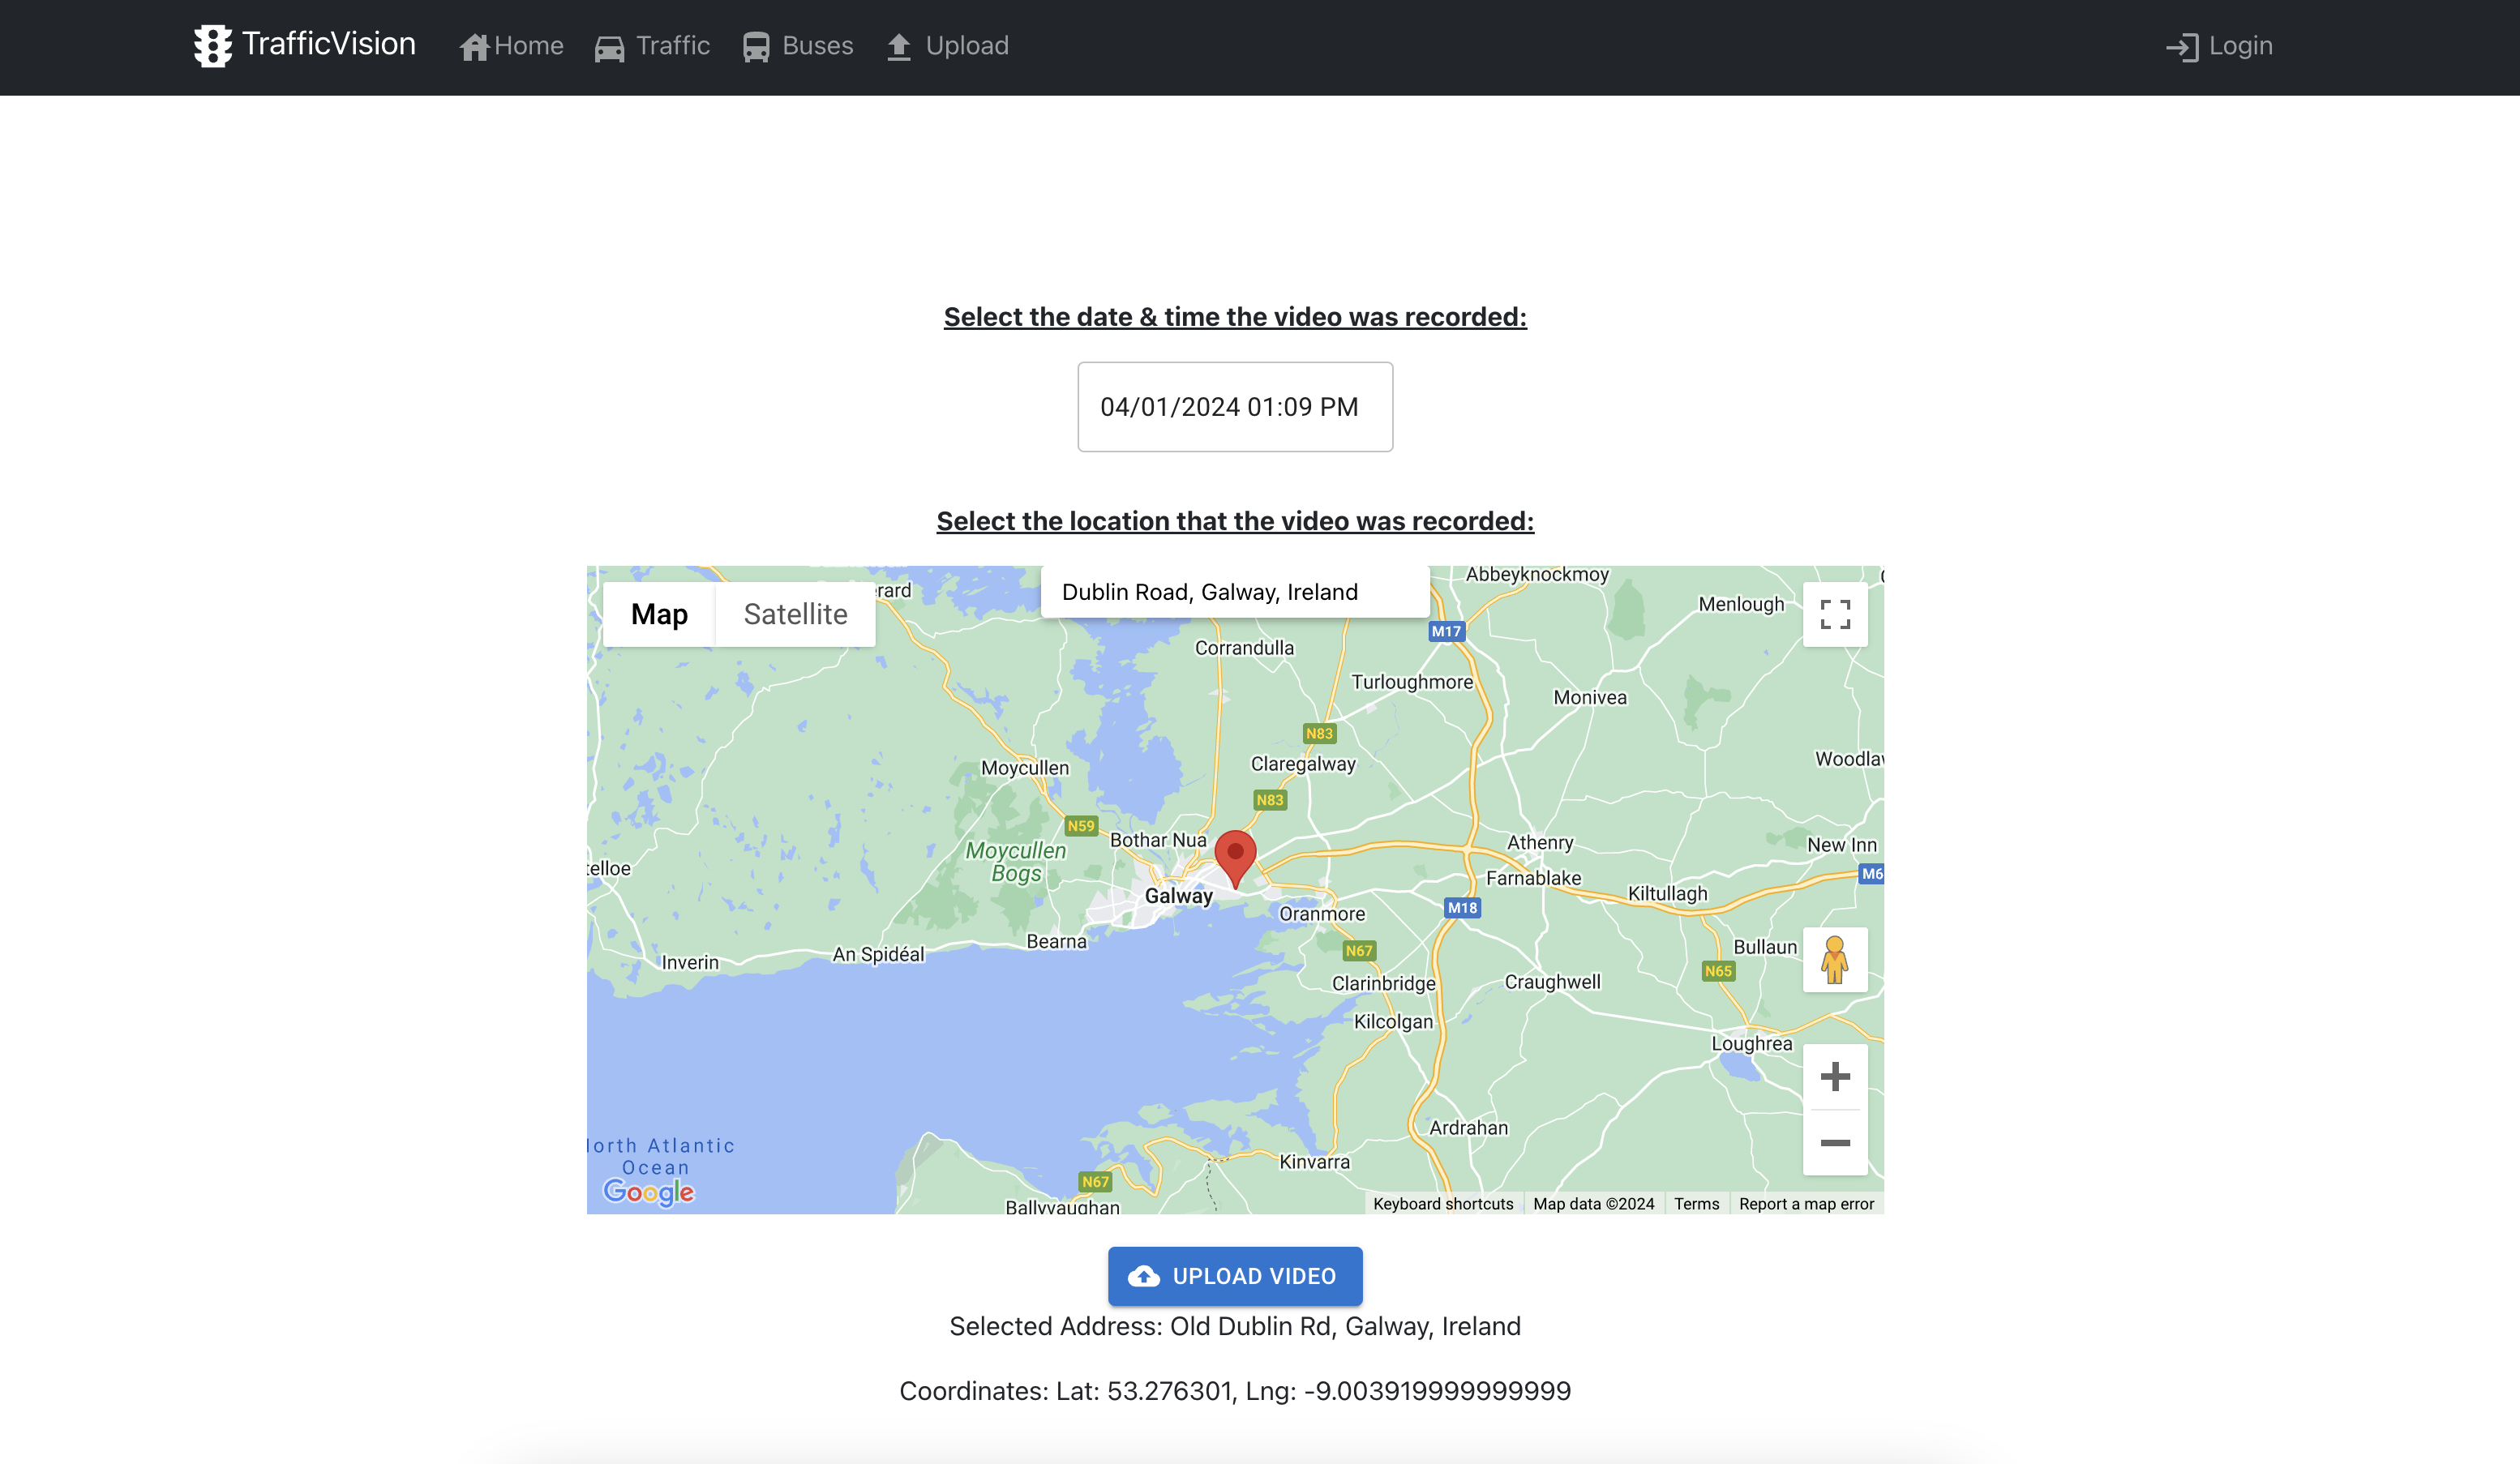
\includegraphics[width=\linewidth]{images/uploadUI.png}
    \caption{TrafficVision's video upload feature, enabling user participation in traffic data crowdsourcing.}
    \label{fig:uploadUI}
\end{figure}

While the system provides a straightforward mechanism for users to contribute data, a notable weakness is the reliance on active user engagement, which may lead to data sparsity. Future enhancements could include gamification elements to incentivize regular contributions or the use of passive data collection methods.

\section{Deployment Challenges}
The TrafficVision system deployment presented significant technical challenges, especially in handling the large scale video processing requirements. The initial deployment strategy used cloud services like AWS which provided extensive resources but had cost and scalability issues due to traffic volumes fluctuating.

To address these concerns, the project shifted toward using Railway\cite{railway2024}, a platform that supports Docker, aiming to simplify the deployment process through containerization. This way we could have a more manageable configuration of our Python applications and dependency management.

Given challenges the challenges met in researching and developing a deployment, the most effective deployment of the TrafficVision system has been on local machines, where video processing can be managed more reliably.

In the future, optimization of the deployment architecture will be a priority, such as stronger cloud offerings or dedicated hardware to handle high video processing. This includes testing machine learning models optimized for resource efficiency and integrating adaptive streaming technologies.

\section{Cross-Platform Development Challenges}
A small team of two members worked on TrafficVision using two different operating systems: Unix and Windows. This configuration introduced special system compatibility and integration issues when using technologies like Confluent for Kafka streams, MongoDB for database management and Python for backend and video processing.

These compatibility issues highlighted the need for development practices that support both environments. The team considered several ways to coordinate their development efforts including:

\begin{itemize}
    \item \textbf{Standardization of Development Tools:} The team focused on using cross-platform compatible tools and technologies to reduce system incompatibility issues. This approach was vital to ensure that all components of the TrafficVision system worked harmoniously across different operating environments.
    \item \textbf{Version Control Systems:} Strong version control practices became critical for effective change management and maintaining system stability across different operating systems. By employing robust version control, the team could manage code changes more efficiently, ensuring that updates did not disrupt the system's operation on any platform.
\end{itemize}

In the future, the team sees the potential in virtual environments integrating into their workflow. Future projects using virtual environments could deliver better development efficiency due to the consistent development settings across systems. This would simplify the development cycle, cut down setup time and reduce compatibility issues.

This experience helped to understand how to work together in a mixed system context, preparing the team for future work involving different development platforms.

\section{Strengths and Weaknesses Summary}
The evaluation of TrafficVision against the set objectives has demonstrated strengths in real-time processing, user interface design and traffic data visualization. Weaknesses are mainly centered around data dependence on user engagement and environmental conditions affecting data acquisition. Addressing these weaknesses will be crucial for the next phase of development, focusing on system robustness and data diversity.

Overall, TrafficVision has made significant strides toward its envisioned goals, laying a solid foundation for future enhancements in traffic monitoring and analysis.